\chapter{Background}
\label{chap:background}

\section{Background}
Based on the previous work of people using NSGA-II on some multi-objective optimization problems\cite{Magnier_2010_Multiobjective}, we believe we can also applied NSGA-II on our Urban Design Model to find the optimal solution. 

\section{Previous Work}

\subsection{Genetic Algorithm(GA)}
After the Genetic Algorithm was introduced in 1975 by John Henry Holland\cite{Holland_1975_Book}, it has been applied in many areas. With mimicking the process of natural selection, GA uses selection, crossover, and mutation to generate solutions and try to find the optimal solution for our problems. More specifically, we have a initial population size, then based on our criterion or objective, we give each individual a fitness value. After we select a certain number of individuals from our population based on their fitness and apply our crossover function with a crossover probability to have some new offsprings. Last, we apply the mutation function with a mutation probability on the new offsprings. Then, we have a new population and repeat our steps until we achieve our optimal solution.

\subsection{Multiobjective Genetic Algorithm(MOGA)}
When we apply GA to find our optimal solutions, we can divide those problems into two categories based on the number of objectives: Single Objective problems and Multi-Objective problems. Let's take a simple example for single objectives first. For example we want to find the minimum value of \(y=x^2\) with \(x\in [-3,3]\), it is easy to see that we could achieve the minimun value at \(x=0\). While, when we have two objectives, problem becomes complicated. For example we want to minimize both \(y_{1}=x^2\) and \(y_{2}=(x-2)^2\). Then we won't be able to find a specific \(x\) value for it. From Firuge 1, any points between \(0\) and \(2\) could be a valid compromise solution. 

\begin{figure}[htp] 
\centering
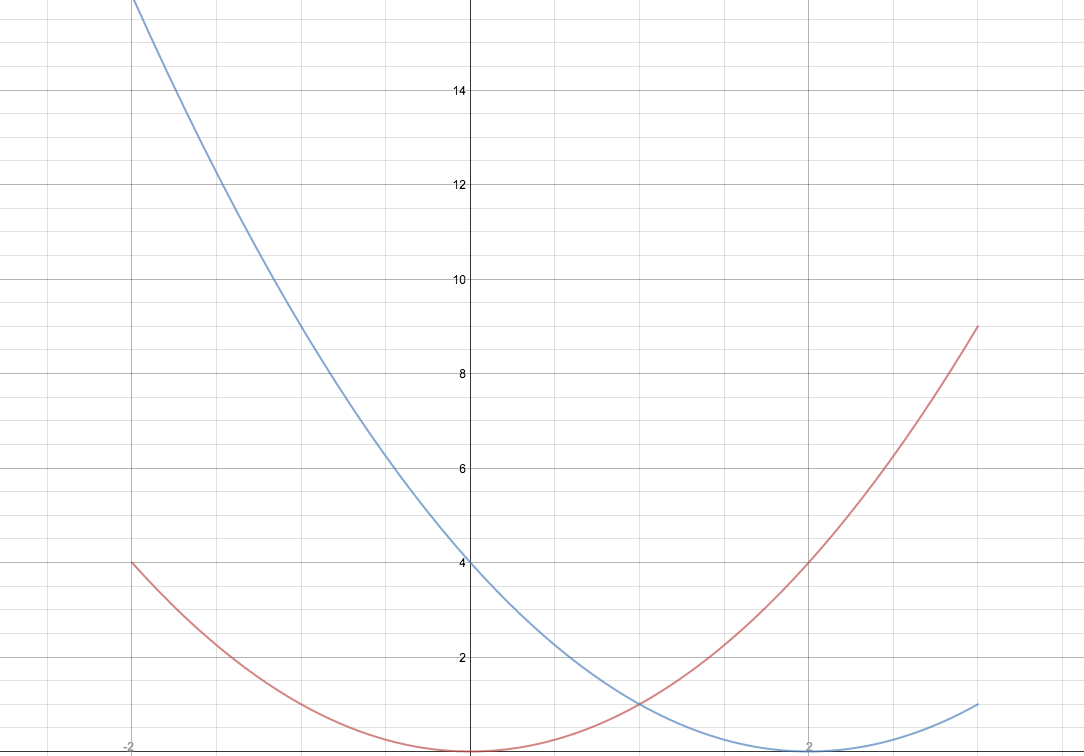
\includegraphics[scale=.4]{images/Figure_1.png}
\caption{Good data.}
\label{fig:goodData}
\end{figure}

In the real word, there are many

\subsection{Nondominated Sorting Genetic Algorithm II(NSGA-II)}
NSGA-II\cite{NSGA-II} is a very famous multi-objective optimization algorithm which is wide used  to find the optimal solution nowadays. Compare with the previous NSGA, NSGA-II has improved the computational efficiency, elitism, and sharing parameter. For computational complexity of nondominated sorting, it improve from \(O(MN^{3})\) to \(O(MN^{2})\). With the elitism, NSGA-II could not only speed up the GA performance, but also prevent loss of good solutions. Moreover, NSGA II does not need to specify a sharing parameter \(\sigma_{share}\), which is a requirement for pervious multi-objective evolutionary algorithms.
